\documentclass[a4paper, 11pt, oneside]{article}

\usepackage[utf8]{inputenc}
\usepackage[T1]{fontenc}
\usepackage[french]{babel}
\usepackage{array}
\usepackage{shortvrb}
\usepackage{listings}
\usepackage[fleqn]{amsmath}
\usepackage{amsfonts}
\usepackage{fullpage}
\usepackage{enumerate}
\usepackage{graphicx}             % import, scale, and rotate graphics
\usepackage{subfigure}            % group figures
\usepackage{alltt}
\usepackage{url}
\usepackage{indentfirst}
\usepackage{eurosym}
\usepackage{listings}
\usepackage{color}
\usepackage[table,xcdraw,dvipsnames]{xcolor}


% Change le nom par défaut des listing
\renewcommand{\lstlistingname}{Extrait de Code}

% Change la police des titres pour convenir à votre seul lecteur
\usepackage{sectsty}
\allsectionsfont{\sffamily\mdseries\upshape}
% Idem pour la table des matière.
\usepackage[nottoc,notlof,notlot]{tocbibind}
\usepackage[titles,subfigure]{tocloft}
\renewcommand{\cftsecfont}{\rmfamily\mdseries\upshape}
\renewcommand{\cftsecpagefont}{\rmfamily\mdseries\upshape}

\definecolor{mygray}{rgb}{0.5,0.5,0.5}
\newcommand{\coms}[1]{\textcolor{MidnightBlue}{#1}}

\lstset{
    language=C, % Utilisation du langage C
    commentstyle={\color{MidnightBlue}}, % Couleur des commentaires
    frame=single, % Entoure le code d'un joli cadre
    rulecolor=\color{black}, % Couleur de la ligne qui forme le cadre
    stringstyle=\color{RawSienna}, % Couleur des chaines de caractères
    numbers=left, % Ajoute une numérotation des lignes à gauche
    numbersep=5pt, % Distance entre les numérots de lignes et le code
    numberstyle=\tiny\color{mygray}, % Couleur des numéros de lignes
    basicstyle=\tt\footnotesize,
    tabsize=3, % Largeur des tabulations par défaut
    keywordstyle=\tt\bf\footnotesize\color{Sepia}, % Style des mots-clés
    extendedchars=true,
    captionpos=b, % sets the caption-position to bottom
    texcl=true, % Commentaires sur une ligne interprétés en Latex
    showstringspaces=false, % Ne montre pas les espace dans les chaines de caractères
    escapeinside={(>}{<)}, % Permet de mettre du latex entre des <( et )>.
    inputencoding=utf8,
    literate=
  {á}{{\'a}}1 {é}{{\'e}}1 {í}{{\'i}}1 {ó}{{\'o}}1 {ú}{{\'u}}1
  {Á}{{\'A}}1 {É}{{\'E}}1 {Í}{{\'I}}1 {Ó}{{\'O}}1 {Ú}{{\'U}}1
  {à}{{\`a}}1 {è}{{\`e}}1 {ì}{{\`i}}1 {ò}{{\`o}}1 {ù}{{\`u}}1
  {À}{{\`A}}1 {È}{{\`E}}1 {Ì}{{\`I}}1 {Ò}{{\`O}}1 {Ù}{{\`U}}1
  {ä}{{\"a}}1 {ë}{{\"e}}1 {ï}{{\"i}}1 {ö}{{\"o}}1 {ü}{{\"u}}1
  {Ä}{{\"A}}1 {Ë}{{\"E}}1 {Ï}{{\"I}}1 {Ö}{{\"O}}1 {Ü}{{\"U}}1
  {â}{{\^a}}1 {ê}{{\^e}}1 {î}{{\^i}}1 {ô}{{\^o}}1 {û}{{\^u}}1
  {Â}{{\^A}}1 {Ê}{{\^E}}1 {Î}{{\^I}}1 {Ô}{{\^O}}1 {Û}{{\^U}}1
  {œ}{{\oe}}1 {Œ}{{\OE}}1 {æ}{{\ae}}1 {Æ}{{\AE}}1 {ß}{{\ss}}1
  {ű}{{\H{u}}}1 {Ű}{{\H{U}}}1 {ő}{{\H{o}}}1 {Ő}{{\H{O}}}1
  {ç}{{\c c}}1 {Ç}{{\c C}}1 {ø}{{\o}}1 {å}{{\r a}}1 {Å}{{\r A}}1
  {€}{{\euro}}1 {£}{{\pounds}}1 {«}{{\guillemotleft}}1
  {»}{{\guillemotright}}1 {ñ}{{\~n}}1 {Ñ}{{\~N}}1 {¿}{{?`}}1
}
\newcommand{\tablemat}{~}

%%%%%%%%%%%%%%%%% TITRE %%%%%%%%%%%%%%%%
% Complétez et décommentez les définitions de macros suivantes :
\newcommand{\intitule}{Polylignes, Milestone 1}
\newcommand{\GrNbr}{06}
\newcommand{\PrenomUN}{Maxime}
\newcommand{\NomUN}{Deravet}
\newcommand{\PrenomDEUX}{Luca}
\newcommand{\NomDEUX}{Matagne}
% Décommentez ceci si vous voulez une table des matières :
\renewcommand{\tablemat}{\tableofcontents}

%%%%%%%% ZONE PROTÉGÉE : MODIFIEZ UNE DES DIX PROCHAINES %%%%%%%%
%%%%%%%%            LIGNES POUR PERDRE 2 PTS.            %%%%%%%%
\title{INFO0947: \intitule}
\author{Groupe \GrNbr : \PrenomUN~\textsc{\NomUN}, \PrenomDEUX~\textsc{\NomDEUX}}
\date{}
\begin{document}

\maketitle
\newpage
\tablemat
\newpage
%%%%%%%%%%%%%%%%%%%% FIN DE LA ZONE PROTÉGÉE %%%%%%%%%%%%%%%%%%%%

%%%%%%%%%%%%%%%% RAPPORT %%%%%%%%%%%%%%%
% Écrivez votre rapport ci-dessous.


\section{TAD: Point2D}

\subsection{Signature}

\noindent TYPE: Point2D

\noindent UTILISE: Réels 

\noindent OPERATIONS: 
\begin{itemize}
    \item Create: Réels $\times$ Réels $\xrightarrow{}$ Point2D {\color{green} C}\footnote{Les lettres vertes permettront, durant tout ce rapport, de mettre en évidence les observateurs et les opérations internes.}
    \item GetX: $Point2D \xrightarrow{}$ Réels {\color{green} O}
    \item GetY: $Point2d \xrightarrow{}$ Réels {\color{green} O}
    \item EuclDist: $Point2D \times Point2d \xrightarrow{}$ Réels {\color{green} O}
    \item Translate: $Point2D \times Point2d \xrightarrow{} Point2D$ {\color{green} T}
    \item Rotate: $Point2D \times Point2d  \times $ Réels $\xrightarrow{} Point2D $ {\color{green} T}
\end{itemize}



\subsection{Sémantique}
\noindent PRECONDITIONS:

\noindent AXIOMES: 
$\forall X,Y \in Reels$
\begin{itemize}
    \item GetX(Create(a,b)) = a
    \item GetY(Create(a,b)) = b
    \item EuclDist(X,Y) = $\sqrt{{(GetX(X)-GetX(Y))}^{2}+{(GetY(X)-GetY(Y))}^{2}}$
    \item GetX(Translate(U,V)) = GetX(U) + GetX(V)
    \item GetY(Translate(U,V)) = GetY(U) + GetY(V)
    \item GetX(Rotate(U,V,f)) = $cos(f) \times (GetX(U)-GetX(V)) - sin(f) \times (GetY(U)-GetY(V)) + GetX(V) $ 
    \item GetY(Rotate(U,V,f)) = $sin(f) \times (GetX(U)-GetX(V)) + cos(f) \times (GetY(U)-GetY(V)) + GetY(V) $ 
    
    
    
\end{itemize}

\subsection{Structure}
Un point est créé sur base du couple de ses coordonnées (x,y). 

\begin{lstlisting}
struct Point2D{
	float x;
	float y;
};
\end{lstlisting}

\subsection{Focntions et procédures}

\begin{lstlisting}[escapeinside={(*}{*)}]

/* 
 * @pre: /
 * @post: (get_x(create_Point2D) = x 
 *(* \color{blue}{$\land$} *)
 * get_y(create_Point2D) = y) 
 */
Point2D* CreatePoint2D(float x, float y);
/* 
 * @pre: A != NULL
 * @post: (*$\color{blue}{A=A_0  \land }  get_x = x$ *)
 */
float get_x(Point2D* A);
/* 
 * @pre: A != NULL
 * @post: (*$\color{blue}{A=A_0  \land }  get_y = y$ *)
 */
float get_y(Point2D* A);
/* 
 * @pre: A != NULL (*\color{blue}{$\land $} *) B != NULL
 * @post: (*$ \color{blue}{A=A_0 \land B=B_0 \land  EuclDist = \sqrt{(X_a-X_b)+(Y_a-Y_b)} } $*)
 */
unsigned float EuclDist(Point2D* A, Point2D* B);
/* 
 * @pre: (*\color{blue}{A != NULL $\land$ B != NULL}*)
 * @post: (*\color{blue}{$A=Translate_{(A, B)} \land B=B_0$}*)
 */
void TranslatePoint2D(Point2D* A, Point2D* B);
/* 
 * @pre: (*\color{blue}{A != NULL $\land$ B != NULL}*)
 * @post: (*\color{blue}{$A=Rotate_{(A, B), x} \land B=B_0 $}*)
 */
void RotatePoint2D(Point2D* A, Point2D* B, float x);
\end{lstlisting}


\section{TAD: Polyligne}

\subsection{Signature}

\noindent TYPE: Polyligne

\noindent UTILISE: Point2D, Réels, Naturels, Boolean


\noindent OPERATIONS: 
\begin{itemize}
    \item Create: $Point2D \times Point2D \times Boolean \xrightarrow{} Polyligne$ 
    \item Close: $Polyligne \xrightarrow{} Polyligne$ {\color{green} T}
    \item Open: $Polyligne \xrightarrow{} Polyligne$ {\color{green} T}
    \item IsOpen: $Polyligne \xrightarrow{} Boolean$ {\color{green} O}
    \item NbrPoint: $Polyligne \xrightarrow{} Naturels$ {\color{green} O}
    \item GetPoint: $Polyligne \times Naturels \xrightarrow{} Point2D$ {\color{green} O}
    \item Length: $Polyligne \times Reels$ {\color{green} O}
    \item AddPoint: $Polyligne \times Point2D \xrightarrow{} Polyligne${\color{green} T}
    \item SuppPoint: $Polyligne \xrightarrow{} Polyligne$ {\color{green} T}
    \item PolyTranslate: $Polyligne \times Point2D \xrightarrow{} Polyligne$ {\color{green} T}
    \item PolyRotate: $Polyligne \times Reels \times Point2D \xrightarrow{} Polyligne$ {\color{green} T}
\end{itemize}

\bigskip

\subsection{Sémantique}

\noindent PRECONDITIONS: $\forall P \in Polyligne, \forall A \in Point2D, \forall x \in Naturels, \forall n \in Boolean$
\begin{itemize}
    \item SuppPoint(P) est défini ssi$2 \leq  NbrPoint(P)$
    \item GetPoint(A,x) est défini ssi $0 \leq x < NbrPoint(P)$
    \item AddPoint(P,A) est défini ssi  $ 2 \leq  NbrPoint(P)$
\end{itemize}

\noindent AXIOMES: $\forall P \in Polyligne, \forall A, B, C \in Point2D, \forall x \in Naturels, \forall n \in Boolean$
\begin{itemize}
    \item Open(Create(A,B,n)) = Create(A,B,n)\footnote{Les Polylignes seeront toujours ouvertes à la création}
    \item Close(Create(A,B,n)) = AddPoint(Create(A,B,False),C)
    \item NbrPoint(Create(A,B,n)) = 2
    \item NbrPoint(AddPoint(P,C, x)) = NbrPoint(P) + 1
    \item NbrPoint(SuppPoint(P, x)) = NbrPoint(P) - 1
    \item NbrPoint(Translate(P, A)) = NbrPoint(P)
    \item NbrPoint(Rotate(P, A)) = NbrPoint(P)
    \item GetPoint(Create(A,B,n), 0) = A
    \item GetPoint(AddPoint(P, C), NbrPoint(P) = C
    \item GetPoint(PolyTranslate(P, C), x) =  Translate(GetPoint(P, x), C)
    \item GetPoint(PolyRotate(P, C), x) =  Rotate(GetPoint(P, x), C)
    \item Length(Create(A,B,n)) = EuclDist(A,B)
    \item Length(P) = $\sum_{x=0}^{NbrPoint(P)-1} EuclDist(GetPoint(P,x),GetPoint(P,x+1))$
    \item Length(Close(P)) = IF( IsOpen(P) = False): Length(P=$P_0$ \footnote{Ici, l'indice "0" est utilisé pour parler de l'état initial de la polyligne, un raisonnement similaire pourrait être utilisé dans le suite du rapport})
    ELSE: Length($P_0$) + EuclDist(GetPoint(P, NbrPoint($P_0$)), GetPoint(P, NbrPoint(P)))
    \item Length(Open(P)) = IF( IsOpen(P) = True): Length(P=$P_0$)
    ELSE: Length($P_0$) - EuclDist(GetPoint(P, NbrPoint($P_0$)), GetPoint(P, NbrPoint(P)))
    \item Length(AddPoint(P)) \& Length(SuppPoint(P))\footnote{Ces deux cas ne sont pas oubliés mais sont bel et bien pris en compte dans les cas "Length(Open(P))" et "Length(Close(P)) car comme nous le verrons, fermer une polyligne ouverte lui ajoute un point (raisonnement opposé pour l'ouverture d'une polyligne" }
    
\end{itemize}



\subsection{Implémentation par tableau}

\subsubsection{Structure}

\begin{lstlisting}
struct Polyline{
	boolean open;
	unsigned nbpoint;
	unsigned arraySize;
	Point2D** pointArray;
};
\end{lstlisting}

L'image ci-dessous est le schéma correspondant à notre structure.

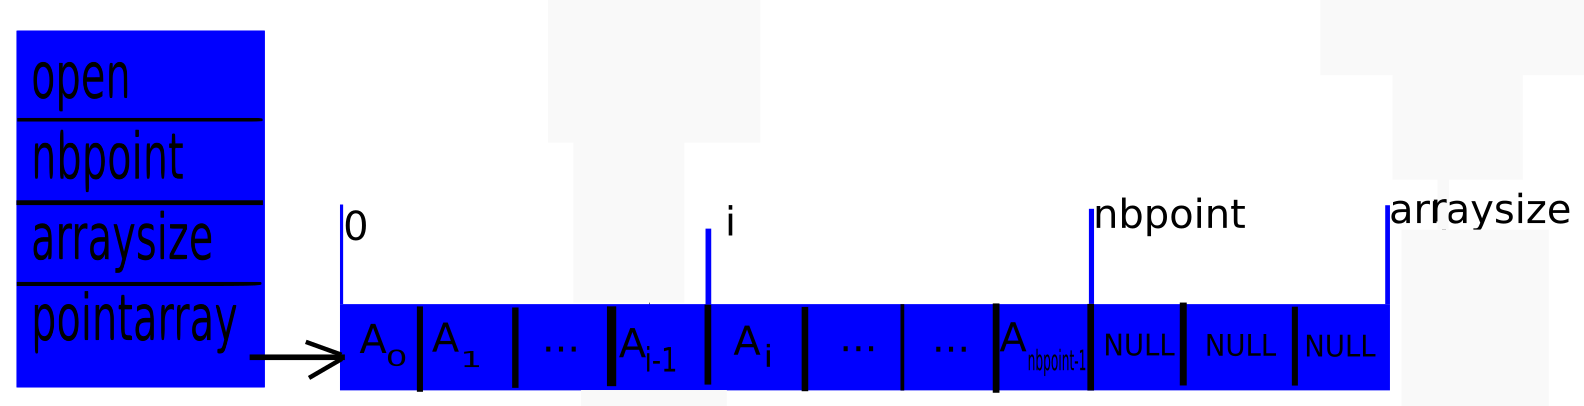
\includegraphics[height=4cm, width=14cm]{tab1.png}

\subsubsection{fonctions et procédures}

\begin{lstlisting}[escapeinside={(*}{*)}]
/* 
 * @pre: A != NULL (*\color{blue}{$\land$} B != NULL \color{blue}{$\land$}*)
 * @post: (*\color{blue}{$A=A_0$ $\land$ $B=B_0$ $\land$ open=open $\land$ create\_Polyligne = P $\land$ }*)
 * (*\color{blue}{nbpoint(P) = NbrPoint(P) $\land$ length(P) = Length(P)}*)
 */
Polyline* CreatePolyline(Point2D* A, Point2D* B, boolean open);
/* 
 * @pre: P != NULL 
 * @post: (*\color{blue}{$P=P_0$ $\land$ open = False $\land$  $nbpoint = nbpoint_0 $*)
 */
void Open(Polyline* P);
/* 
 * @pre: P != NULL 
 * @post: (*\color{blue}{$P=P_0$ $\land$ open(P) = True $\land$ $nbpoint = nbpoint_0 $ *)
 */
void Close(Polyline* P);
/* 
 * @pre: P != NULL 
 * @post: (*\color{blue}{$P=P_0$ $\land$*)
 */
void IsOpen(Polyline* P);
/* 
 * @pre: P != NULL
 * @post: (*\color{blue}{P=P$_0$ $\land$} nbpoint = NbrPoint(P) *)
 */
unsigned NbrPoint(Polyline* P);
/* 
 * @pre: (*\color{blue}{$P != NULL  \land$ } numero < nbpoint*)
 * @post: (*$\color{blue}{P=P_0 \land} GetPoint = {A_{numero}}$*)
 */
Point2D GetPoint(Polyline* P, unsigned numero);
/*
 * @pre: (*\color{blue}{ P != NULL $\land$ A != NULL }*)
 * @post: (*\color{blue}{$A=A_0$ $\land$ $open =open_0$ $\land$} \color{blue}{$nbpoint = nbpoint_0 + 1$  *)
 */
void AddPoint2D(Polyline* P, Point2D* A);
/*
 * @pre: (*\color{blue}{ P != NULL $\land$ A != NULL }*)
 * @post: (*\color{blue}{$A=A_0$ $\land$ $open =open_0$ $\land$} \color{blue}{$nbpoint = nbpoint_0 - 1$  *)
 */
 void SuppPoint2D(Polyline* P);
\end{lstlisting}

Les fonctions et procédures reprisent ci-dessus ne nécessitent pas d'invariant spécifique. On pourrait imaginer qu'il en faut un pour l'ajout et la suppression d'un point mais nous prenons la décision de n'ajouter et de supprimer que le dernier point à chaque appel de cet fonction. Le seul élément de l'ajout/la suppression d'un point qui pourrait encore nécessiter un invariant est le calcul de la longueur de la polyligne. Une fonction étant totalement dédiée à ce clacul, nous allons présenter l'invariant pour celle-ci. 

\subsubsection{Invariant et spécifications: Length}

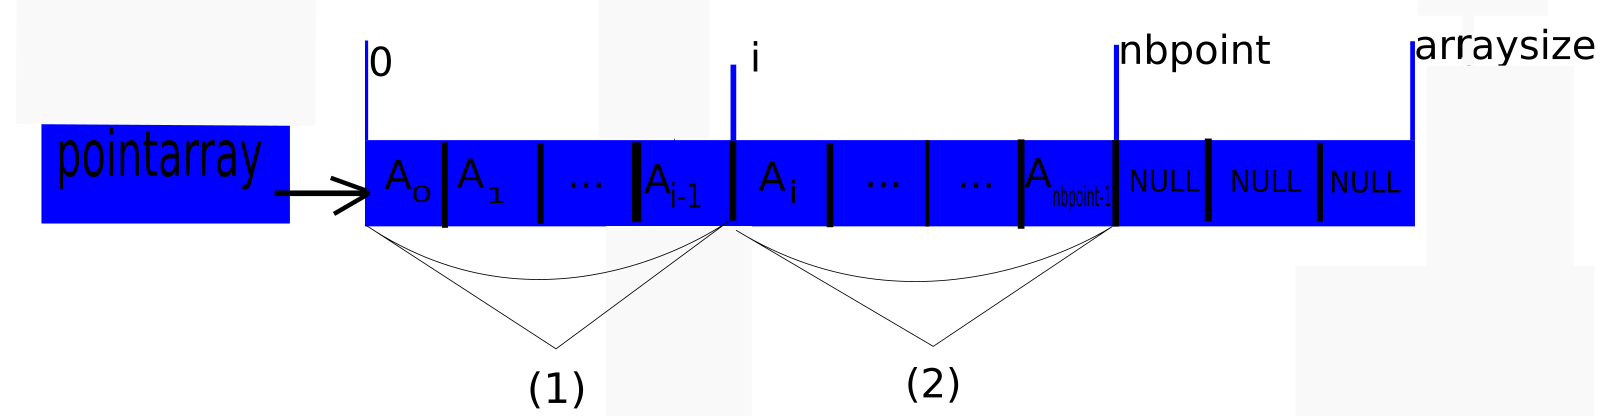
\includegraphics[height=4cm, width=14cm]{inv1.png}

(1): Length = $\sum_{x=0}^{i-2} EuclDist(A_x,Ax+1)$

(2): Length à calculer

\noindent L'invariant formel qui en découle est le suivant:

\noindent$ pointArray = pointArray_0 \land \forall x, 0\leq x \leq i-2, Length =\sum_{x=0}^{i-2} EuclDist(A_x,Ax+1) \land arraySize = arraySize_0 \land nbpoint = nbpoint_0 $

\smallskip



\begin{lstlisting}[escapeinside={(*}{*)}]
/*
 * @pre: (*\color{blue}{ P != NULL}*)
 * @post: (*\color{blue}{$P=P_0$ $\land$ $Length=\sum_{x=0}^{NbrPoint(P)-1} EuclDist(GetPoint(P,x),GetPoint(P,x+1)) $}
 *)
 */
 float Length(Polyline* P);
\end{lstlisting}

\subsubsection{Invariant et spécifications: PolyTranslate}

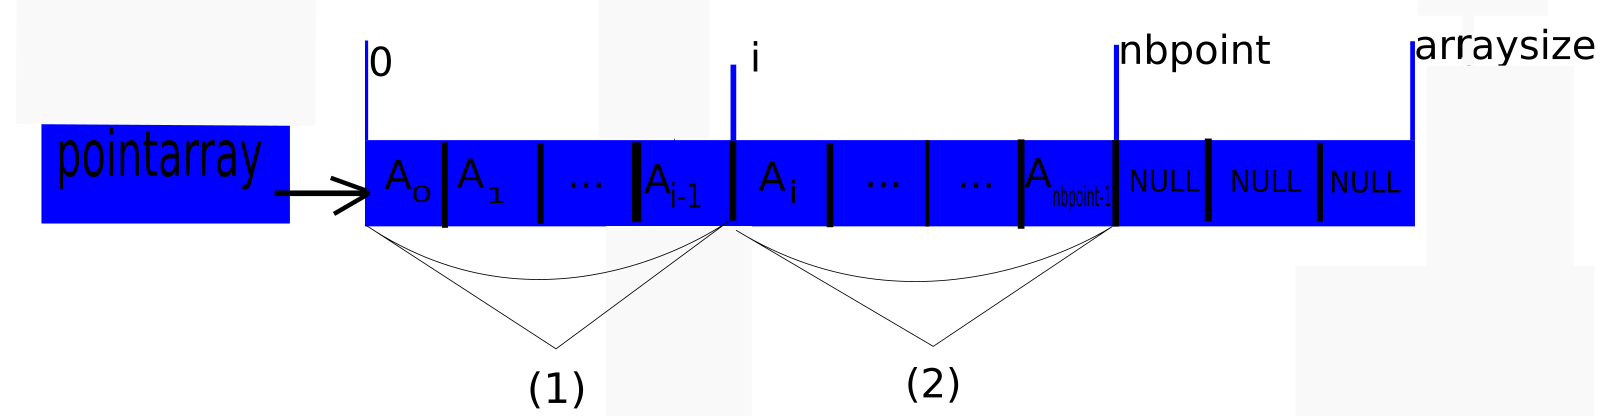
\includegraphics[height=4cm, width=14cm]{inv1.png}

(1): La translation de chaque point est effectuée

(2): Translation à appliquer sur les points restants

\noindent L'invariant formel qui en découle est le suivant:

\noindent$ \forall x, 0\leq x \leq i-1, A_x = Translate((A_x)_0, K)\footnote{K est le point de référence lors de cette Translation})  \land arraySize = arraySize_0 \land nbpoint = nbpoint_0 $

\smallskip



\begin{lstlisting}[escapeinside={(*}{*)}]
/*
 * @pre: (*\color{blue}{ $P != NULL \land K != NULL$} *)
 * @post: (*\color{blue}{$P=P_0$ $\land$ $C=C_0 \land  \forall x, 0\leq x \leq i-1, A_x = Translate((A_x)_0, K)  $}
 *)
 */
 void PolyTranslate(Polyligne* P, Point2D K);
\end{lstlisting}


\subsubsection{Invariant et spécifications: PolyRotate}

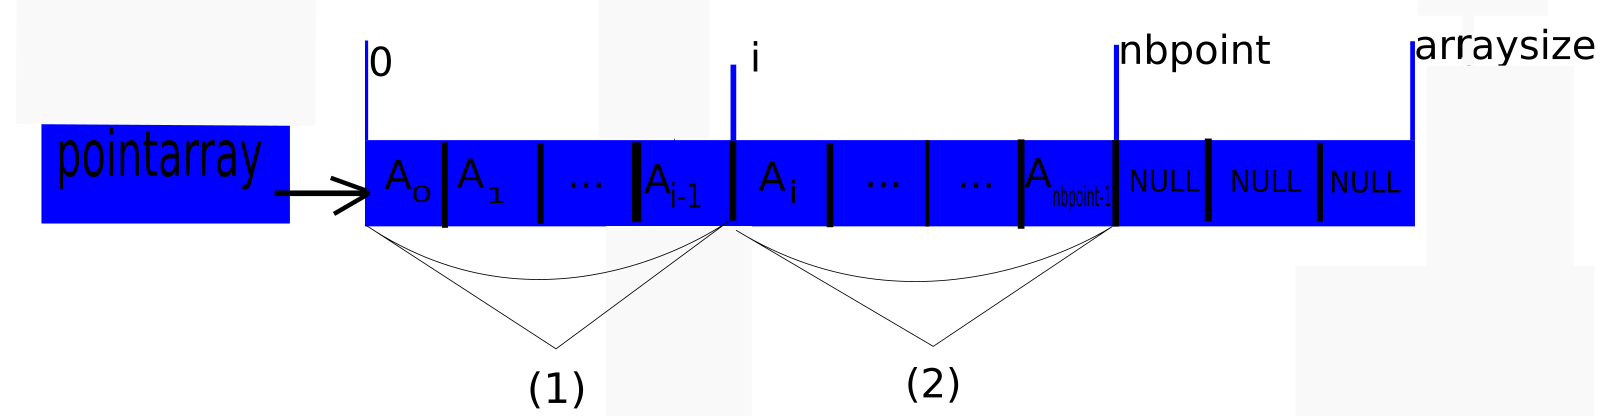
\includegraphics[height=4cm, width=14cm]{inv1.png}

(1): La rotation de chaque point est effectuée

(2): Rotation à appliquer sur les points restants

\noindent L'invariant formel qui en découle est le suivant:

\noindent$ \forall x, 0\leq x \leq i-1, A_x = Rotate((A_x)_0, K)\footnote{K est le point de référence lors de cette Rotation})  \land arraySize = arraySize_0 \land nbpoint = nbpoint_0 $

\smallskip

\begin{lstlisting}[escapeinside={(*}{*)}]
/*
 * @pre: (*\color{blue}{ $P != NULL \land K != NULL$} *)
 * @post: (*\color{blue}{$P=P_0$ $\land$ $C=C_0 \land  \forall x, 0\leq x \leq i-1, A_x = Rotate((A_x)_0, K)  $}
 *)
 */
 void PolyRotate(ePolyligne* P, Point2D K);
\end{lstlisting}

\subsection{Implémentation par liste chainée}

\subsubsection{structure}

La structure Point2D est déjà définie plus haut mais il  est important de préciser qu'inclure cette structure(Point2D) dans une liste chaînée nécessite de définir une nouvelle structure. 

\begin{lstlisting}
struct Point{
    Point* prec;
    2DPoint* point;
    Point* suiv;
};
\end{lstlisting}


Dans la liste chaînée gérant la polyligne, nous décidons de garder la longueur et le nombre de point dans une cellule d'en-tete afin d'y accéder plus facilement.
\begin{lstlisting}
struct Polyline{
	char open;
	unsigned nbrpoint;
	unsigned float length;
	Point* head;
};
\end{lstlisting}

Voici un schéma représentant le structure polyligne implémentée par une liste chaînée.

\includegraphics[height=4cm, width=14cm]{schemalist.png}

\subsubsection{Fonctions et procédures}

Les spécifications des fonctions et des procédures sont semblables à l'implémentation par tableau, nous allons juste reprendre deux schémas qui expliquent le fonctionnement des fonctions qui nécessitaient un invariant. Deux schémas et non trois car la longueur de notre polyligne sera stockée dans la cellule d'en tëte de notre liste. Il ne sera donc plus nécessaire de parcourir toute la liste afin de la calculer

\paragraph{AddPoint}
\smallskip

Souvenons nous que notre fonction d'ajout va ajouter notre nouveau point à la fin de la liste. les étapes pour cela seront les suivantes:
\begin{itemize}
    \item[1] Amener l'élément courant au dernier élément de  la liste
    \item[2] Initialiser le champ "suiv" de la nouvelle cellule vers la première de la liste
    \item[3] Initialiser le champ "prec" de la nouvelle cellule vers l'élément courant
    \item[4] Stocker l'adresse de la nouvelle cellule dans dans le champ "suiv" de l'élément courant
    \item[5] Stocker l'adresse de la nouvelle cellule dans le champ "prec" du premier élément de la liste
\end{itemize}

\includegraphics[height=4cm, width=14cm]{schemaadd.png}


\paragraph{SuppPoint}
\smallskip

Souvenons nous que notre fonction d'ajout va ajouter notre nouveau point à la fin de la liste. les étapes pour cela seront les suivantes:
\begin{itemize}
    \item[1] Amener l'élément courant au dernier élément de  la liste
    \item[2] Changer le champ "suiv" de l'avant dernier élément pour le champ "suiv" de l'élément courant
    \item[3] Initialiser le champ "prec" du premier élément pour le champ "prec" de l'élément courant
    \item[4] supprimer l'élément courant
\end{itemize}




\includegraphics[height=4cm, width=14cm]{schemasupp.png}

\section{Complexité}



\section{Comparaison des implémentations}

\end{document}
